\documentclass[a4, UTF8]{article}
\usepackage{amsmath}
\usepackage{bm}
\usepackage{hyperref}
\usepackage{graphicx}
\begin{document}
\title{List of remarks and minor corrections\\
\large ``Interplay between Complex Orders in Functional Materials''\\
by\\
Dott Louis Ponet, Scuola Normale Superiore}
\date{}
\maketitle
I thank the referee for his time, and the quality of the comments and suggestions in order to improve the thesis.
In what follows below, I have compiled the list of remarks each with my reply or explanation, and the possible changes that I made to the thesis as a result.
\\\\
{\bf Page 10:}~{\it The candidate states: ``Without loss of generality, we choose this point to be the gamma point.'' This does not appear to be obvious, because not all T-invariant points are equivalent. Can this be better explained?}
\\\\
% This is true. What is meant here is that for the purpose of the derivation only $\bm k_r = \bm k - \bm \bm k_0$ matters. Whether $\bm k_0 = \bm 0$ or another T-invariant point changes what the $|u_n, \sigma>$ are in Eq.(2.14).
{\bf Page 17:}~{\it Why is the exact experimental unit cell not used in this case? Is the unit cell used here the result of DFT optimisation?}
\\\\
No particular reason.
\\\\
{\bf Page 24, Fig.~2.9:}~{\it The direction of the path in reciprocal space is not clear on the axes.}
\\\\
I have added $A \leftarrow Z \rightarrow U$ to this and the following figure.
\\\\
{\bf Page 36, Fig.~3.1:}~{\it This figure is not at all clear, partly due to the fact that only few spin directions are indicated. One should first of all sttate in the caption that the chains are AFM, but also indicate some of the spins so that the fragments in panels b) and c) can be identified in the larger structure.}
\\\\
Thank you for this suggestion, I have added the spins corresponding to b) and c) in a).
I have also added a more explicit statement of the AFM nature of the chains in the caption.
\\\\
{\bf Page 37:}~{\it The candidate states that the electronic and lattice polarisations largely cancel in other members of the $R$Mn$_2$O$_5$ family but not in GdMn$_2$O$_5$. This is a bit of an exaggeration, as the polarisation in GdMn$_2$O$_5$ is not hugely different from YMn$_2$O$_5$, for example - perhaps restate.}
\\\\
This was my mistake, I misinterpreted some discussions on the comparison of ab-initio calculations on $R$Mn$_2$O$_5$, either neglecting or including on-site Coulomb repulsion, where it was shown that without including correlations the polarization is an order of magnitude larger (see e.g. \href{https://arxiv.org/abs/0802.0653v1}{Electronic correlations decimate the ferroelectric polarization of multiferroic HoMn$_2$O$_5$}). However this happens in{\it any} $R$Mn$_2$O$_5$, making my wording misleading at best. I have changed it to be more precise, refering to the above paper. 
\\\\
{\bf Page 38, Fig.~3.2:}~{\it It is really a pity that panel a) is inconsistent with previous measurements and with theory. Have these measurements been repeated?}
\\\\
Up to this point in time, sadly not. We are still not entirely sure why this is happening, since the samples are identical as far as we know, and it is simply not possible to get the four-state behavior without having both two-state behaviors. We are currently working together with the experimentalists to further understand what might be causing this and further interesting effects.
\\\\
{\bf Page 39, Fig.~3.3:}~{\it Some of the magnetic field scales are missing.}
\\\\
Fixed
\\\\
{\bf Page 44 and following:}~{\it The analysis provided in terms of individual spins is adequate but
inelegant. In general, this type of analysis is better done in terms of Fourier components with
terms properly related by symmetry via irrep transformations, leading to a set of order parameters.
For example, in the absence of a magnetic field, it is clear that Gd spins must transform with the
same irrep as Mn spins in order for coupling to exist. There may be a good reason why this is not
possible or convenient here – explain.}
\\\\
Initially we tried to indeed construct a model using this method, based on the description in the middle of page 3 of \href{https://link.aps.org/doi/10.1103/PhysRevLett.110.137203}{Giant Tunability of Ferroelectric Polarization in GdMn$_2$O$_5$}. This means we used the X$_2$ irrep and its modes to find the invariants. We found that this led to very complicated expressions and we made little progress through this way, after which we decided to try it in this more explicit way.
After finding that the model very well described the experiments, we tried to project the components of the spins and N\'eel vectors onto the X$_2$ modes during a field sweep. This is displayed in figure \ref{allirreps}.
\begin{figure}[h]
	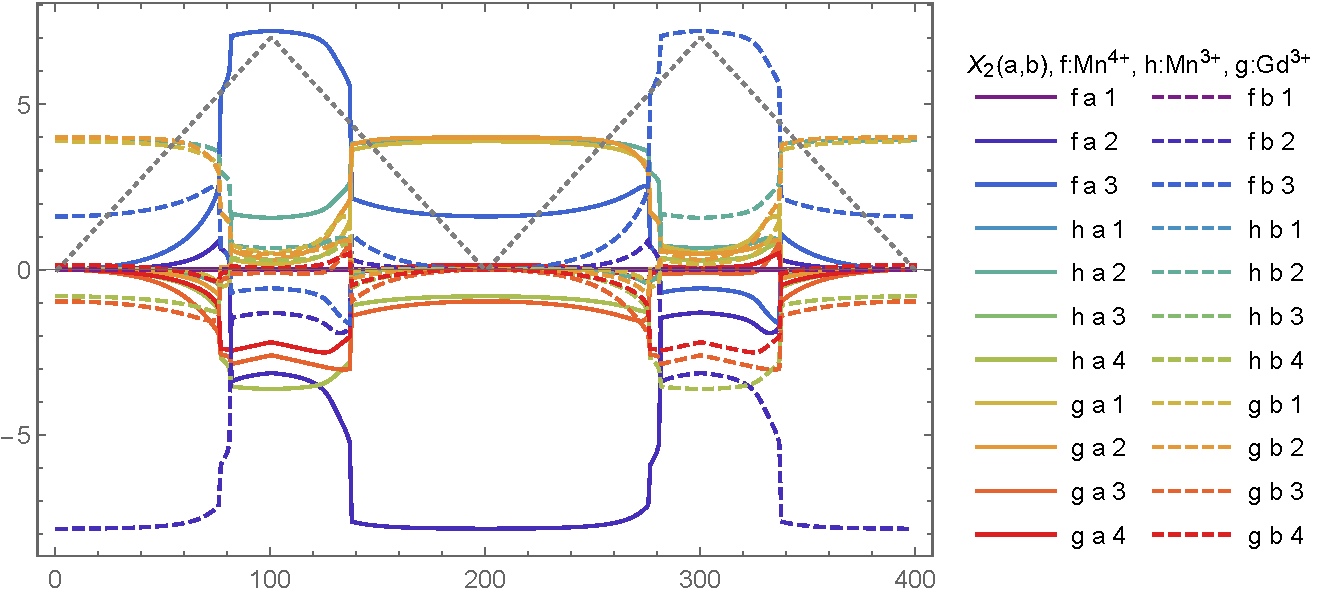
\includegraphics[width=\textwidth]{allIrreps.pdf}
	\caption{\label{allirreps}{\bf Projections onto X$_2$ modes.} The graphs represent the projections on the (a,b) components of the X$_2$ of the spins that are in the unit cell, during the double field sweep. The magnetic field amplitude is represented by the grey dotted graph. The three Wyckoff positions are labeled by $f$, $h$ and $g$ for the Mn$^{4+}$, Mn$^{3+}$, and Gd positions. The numbering denotes which spatially equivalent Wyckoff position the moment belongs to, and the full and dotted graphs denote the $a$ and $b$ components of each moment, respectively.}
\end{figure}
From the figure it is clear that the behavior of the projections of the spins is rather complex, and many require the full 2D projections to describe their evolution throughout the full cycle.
Our model is greatly simplified since, through the use of the unit vectors in the $ab$ plane, we have only one angle per spin as the variable.
\\\\
{\bf Page 50:}~{\it The candidate mentions the Nudged Elastic Band model which, however, is not introduced.}
\\\\
I have added a small description to the text:\\
``The Nudged Elastic Band calculations are a way to track how the low points of the valley in Fig.~\ref{fig:GdMn2O5_heatmap} change for different field strengths.
This is done by taking two extremal states, then constructing a set of images that interpolate in phase space between these two states. The total energy of the entire chain is then optimized using a small elastic-like energy term that binds the images together, so that they find the lowest energy barrier between the two states.''
\\\\
{\bf Page 54, Fig.~3.10:}~{\it I found this figure (especially the `squiggles' in panels b to f) extremely confusing. I am not sure it adds much, so I would consider omitting, but a better caption is certainly in order.}
\\\\
This figure was made in an attempt to summarize all the possible switching behaviors that can be observed in the material, depending on the field orientation. The squiggles are a way to demonstrate how the evolution of the AFM order parameters happens when the field is swept up and down, with the color gradient of panel (a) encoding the time evolution, which corresponds to the gradient of the squiggles.

I have changed the caption in an attempt to be more clear.
\\\\
{\bf Page 65, Fig.~4.1:}~{\it The discussion of the diffraction data, especially panel b) is rather confusing:
what are the ‘blobs’ we are looking at (finite-size fringes mixed with superlattice peaks?) This may
be clear from the related publications but not here.}
\\\\
I have added a little more explanation in the main text, updated the schematic figure in panel (b), and added additional information to the caption of the figure.
\\\\
{\bf Page 66, Fig.~4.2:}~{\it Perhaps a qualitative introduction to panel a) in this figure could help. I now understand what is going on, but I must admit it took me a while. Also, please provide the
reference to the publication in the figure caption, both here and elsewhere.}
\\\\
I have added the following qualitative description to the main text:

``We first focus on Fig.~4.2(a), where the PLD amplitude is represented as a heatmap with on the x-axis the time evolution, and on the y-axis the delay between the two consecutive pumps by optical pulses. The y-axis basically shows many experiments such as the ones in panel (b) and (c) of the same figure. Consequently, the blue and purple line demonstrate the horizontal slice corresponding to the measurement highlighted by the box with the same color.''

The publication with the figure is in the final stages of publishing, I will add the reference as soon as it is fully accepted.
\\\\
{\bf Page 67, Fig.~4.3:}~{\it The caption states `The dashed red line marks...’ but there are two dashed red lines...}
\\\\
It should have been plural. This panel is meant to demonstrate that when the first pulse is so intense that it heats the material so much that the order never restores, the different timings of the second pulse (i.e. the two dashed lines) has little to no effect, contrary to when the order is allowed to (partially) restore.
I have corrected this in the caption.
\\\\
{\bf Page 68:}~{\it There is a rather cryptic reference to `topological defects' - please explain.}
\\\\
I have expanded the discussion to:

``Finally, it was experimentally verified that no timescales related to the behavior of topological defects such as domain walls are present. This would be reflected in a changing width and intensity of the diffraction peaks associated with the PLD (Fig.~1.1(b)), which is not observed. This can be explained by the small thickness of the film, allowing only a single SDW wavevector direction, such that no domains are formed in the ``depth'' of the film. Furthermore, the XFEL pulses had a diameter of 0.2 mm, w hich envelopes multiple SDW domains in the plane of the film [Nicholson2016], making the measurements statistical over domains.
These considerations also support our previous claim that the optical pulses can be assumed to excite the thin film homogeneously.''
\\\\
{\bf Page 80:}~{\it I found the introduction to Chapter 5 rather unsatisfactory. Why is the problem of FE soft domain walls interesting/relevant (i.e., who cares)? The link to the possibility of using the described effect for information storage seems rather remote. It would be much preferable if a
higher-level context was provided.}
\\\\
{\bf Page 82:}~{\it ``The longitudinal part... leads to the largest contribution...''. How universal is this statement? Is that `usually'?}
\\\\
Indeed, looking at Table II in \href{http://dx.doi.org/10.1063/1.4861260}{Electrostrictive effect in ferroelectrics: An alternative approach to improve piezoelectricity}, the fluorites have a larger shear electrostrictive coefficient. I have changed it to `usually' in the text.
\\\\
{\bf Page 83:}~{\it In the absence of a higher-level context generalising the importance of the problem, I found the introduction to the experimental section a rather satisfactory substitute – in other words, the candidate’s collaborators found some unusual results experimentally and asked for help!
Perhaps there is scope to move this introduction higher up.}
\\\\
{\bf Page 84:}~{\it The reference to the `measure of the noise’ is unclear.}
\\\\
What was meant is that since only out-of-plane components of the polarization are measured in these experiments, any in-plane polarization would result in the same angle denoted by the coloration. The variations in the color then rather demonstrate the noise of the measurement technique, since it should be a uniform color if the measurements were perfect. I've added some additional discussion on this in the text.
\\\\
{\bf Page 85, Fig.~5.2:}~{\it The order of the panels seems confusing. Panel e) should be moved next to
panel c) for consistency with a) and b). Panels d) and f) do not add much but they could go on the
bottom.}
\\\\
Yes that makes much more sense, I've changed it.
\\\\
{\bf Page 87:}~{\it ``It was found that the contribution Delta Z due {\bf to} hybridization'' it is just about the only typo that I could find in the {\bf whole} thesis.}
\\\\
Fixed. Indeed, Grammarly is truly fantastic.
\\\\
{\bf Page 89, Tab~5.1:}~{\it It is not clear where the parameters come from. Were they obtained from the literature or from the candidate’s own work?}
\\\\
These were all taken from previous literature, I have added that and the references.
\\\\
{\bf Page 96:}~{\it The `spurious numerical effect' used in lieu of the P-N barriers seems rather
unsatisfactory and poorly controllable. Can the candidate describe a possible alternative?}
\\\\
\end{document}
